\chapter{A discussion of extensions}\label{chapter-extensions}
%Future work
Our model has been developed to be extensible. In the development of the model we have constantly considered how to integrate the most likely and most useful extensions. In this chapter, we briefly describe a number of those extensions, what we might learn from them, and how we propose to incorporate them,



\section[Amenity]{Incorporating amenity}\label{section-amenity}
% from Ricardo_Rent_and_Roemer_3.tex
In our base model,  an urban wage premium is the only labour attractor: it an the transportation cost determine land values. In our base version therefore, we have set the level of amenities to zero  so we can focus on the productivity effects. The wage premium provides a reason to find housing in the city and to travel to the city centre to work. Housing choice, however, is always the purchase of a bundle of characteristics such as location, building space, yard, local density and local \glsdisp{amenity}{amenities}. Stegman  found that ``a large majority of families who have recently moved to the suburbs are more concerned with neighborhood quality than with accessibility to other parts of the metropolitan region.'' 
``There is evidence that the amenities offered by a city enhance its growth \cite{clarkAmenitiesDriveUrban2002, falckPhantomOperaCultural2011a} and that amenity effects themselves scale superlinearly\cite{kraemerCulturalSustainabilityUS2022}. 



Kaufmann et all \cite{kaufmannScalingUrbanAmenities2022} investigated the general statistical patterns in the quantity and spatial distribution of different urban amenities including public spaces and institutions as well as businesses, which all provide different services to urban populations, such as restaurants, parks, or universities.  They argue that amenities are   in fact central for generating and supporting economic agglomeration effects, attracting investment to ``developing neighborhoods, promoting economic growth, supporting innovation clusters and facilitating businesses linkages.'' 
They show that the aggregate quantity of amenity infrastructure (not amenity supply)  in an urban area scales sub-linearly with population size across US metropolitan areas.\footnote{When they disaggregate, however, they find that for approximately 74\% of amenity types, they cannot reject linear scaling. Four percent exhibit super-linear scaling. They list take-away restaurants and travel agents in this range. Sub-linear scaling is associated with libraries, universities, and movie theatres.} This strongly suggests there are scale economies in amenity provision.\footnote{The model they use is the same as the one used to demonstrate that a scaling law holds for urban GDP. Instead of GDP, however, the dependent variable is a measure of amenity density based on data extracted from a unique new Google Places dataset, Google Places API (2012).} 


The amenities offered by a city can be seen as a form of non-market, non-monetary income. \cite{kaufmannScalingUrbanAmenities2022}.  The non-market component of household incomes affects choices. Greater consumption amenities in a city will make workers willing to accept lower wages or higher rents. For firms,  lower wages mean lower costs. Thus,  higher amenity levels may lead to lower money wages as workers trade amenity for money income. With lower wages, more workers can be hired leading to higher output and a larger population. \cite{pugaMagnitudeCausesAgglomeration2010}. 
When positive urban amenities prevail, rents and housing prices will be higher in larger cities, but wages may be unaffected \cite{robackWagesRentsAmenities1988, dalmazzoAmenitiesSkillbiasedAgglomeration2011}.
%localized productive advantages will make firms willing to accept higher wages and higher rents  


%It involves budget allocation. If we hold the housing budget constant and add an explicit urban amenity, other variables must adjust. 
% Higher wages make residents better off whereas higher rents make them worse off. Thus, 


%.  This helps disentangle the consumption amenities from the productive advantages of big cities.


In our base model,  To introduce amenities we can simply add an amenity value $A$ to the estimated value of any home. The value can depend on location, allowing for `better' and `worse' neighbourhoods,  and it can be made to depend on household attributes: a family with children might value a neighbourhood with a school or a park more highly. 

For some households, the amenity of an area may depend on the density of the city or of certain types in a neighbourhood. This is a social agglomeration effect that may work in addition to the agglomeration effect on production (\cite{gurwitzCatastrophicAgglomeration2019}) that we have already considered. There are also agglomeration effects in consumption goods. Larger consumer markets support more variety in goods and services. This variety allows a greater range of preferences to be satisfied. A larger city may have more production sectors and a larger array of consumer services, increasing the value received from a given income.  These closely related but different effects can be modeled by introducing an amenity term in various ways 

The amenity-induced rise in housing prices may absorb what would otherwise be consumption expenditure on other goods. Residents might accept smaller housing units for access to urban amenities. \footnote{Some costs may fall with agglomeration. There is evidence of a strong negative correlation between the total energy consumption of a city and its overall urban density \cite{NewmanPeterJeffrey}. Larson et al. \cite{larsonEnergyImplicationsCity2015} show that per-capita energy use is relatively invariant to city size when growth is driven by wages but falls modestly with growth induced by rising amenity.} In any case, there will be distributional effects as amenities play a larger role in urban agglomeration. Property owners will capture increased land rents. If amenities are funded out of taxes, the burden falls on all residents, since property taxes are very roughly related to housing consumption, but the land rents are captured by institutional owners as well as owner-occupiers and not by tenants.
÷

%\glspl{amenity}, or non monetary income it another form of wealth,See Kaufmann et al. \cite{kaufmannScalingUrbanAmenities2022}.  and it is %, are however, an important feature of the urban system. 
% We have intentionally suppressed amenity but can add it it simply.
% (ownership effects, produtivity spilllovers, - table where you show them in the static and dynamci case with amentity)
% 2 classes of exploratin of the model in the past tho chaptered
 This sectionr sketches an extension of the model to study include \gls{amenity} and suggests how it might affect results. 

 
%To understand amenity in our model, we need to understand it's relationship with growth, productivity, and agglomeration.
\subsection{Modelling amenity}
Amenity effects can be introduced in a variety of ways. hey might work though An economics might prefer to introduce amenity as a good in the utility function of agents. It might then depend on the size of the city, the size of an amenity-producing sector, the specific amenity-generating infrastructure provided by the city through taxes,  or neighbourhood effects. Each of these would take a different functional form. In our model agents are represented by their demand for housing, so the same terms would have to be introduced into the bid function. In the utility framework, bids are simply derived from the utility function, so the two approaches are equivalent. The virtue of using the utility framework is that it begins with the question, "What do people want?" rather than "What do people do?" The first question is more productive if we want to identify different amenities that might matter.

\subsubsection{Through household utility}
 The most direct way to incorporate agglomeration amenities is to include what might be called a \gls{utility premium} for urban dwellers as non-monetary location income $\mathbb{A}(d; N), \die{\mathbb{A}}{N}> 0), \die[{\mathbb{A}}]{d}< 0)$ depending on distance, $d$ from the centre and urban population $N$. The second term can incorporate local amenities as well. A simple linear (indirect)\footnote{The indirect utility function is a function that depends on income and prices rather than goods and services.  Income does not generate utility, but it does generate utility indirectly' because it enables people to purchase goods and services.} utility function specified on broad income (net wage plus locational amenity) is convenient for illustration:

\begin{equation}VU(w,A)= \psi+ \omega-cd + \mathbb{A}(d; N) - T(d))
\label{eqn-u}
\end{equation}
where $w$  is an urban wage p, $T(d)$ is transportation cost from the centre to $d$.
\footnote{\cite{anasUrbanSpatialStructure1998} shows that a linear transportation cost will not  hold if congestion declines  with $d$.} 
 In most versions of the Alonzo model the `wage premium' is simply given in the urban wages and there is no amenity term. 


%\footnote{wage income, if all income goes to housing, or the share of wage income going to housing services.   (If we use a Cobb-Douglas utility function we would just replace $w$ with    $\alpha Y$, where $Y$ is household income and $\alpha$ is the share of total income. } Let  $T(d)=td$ be transportation cost with  $t>0$. 
 
\begin{figure}[t!b]
\begin{center}
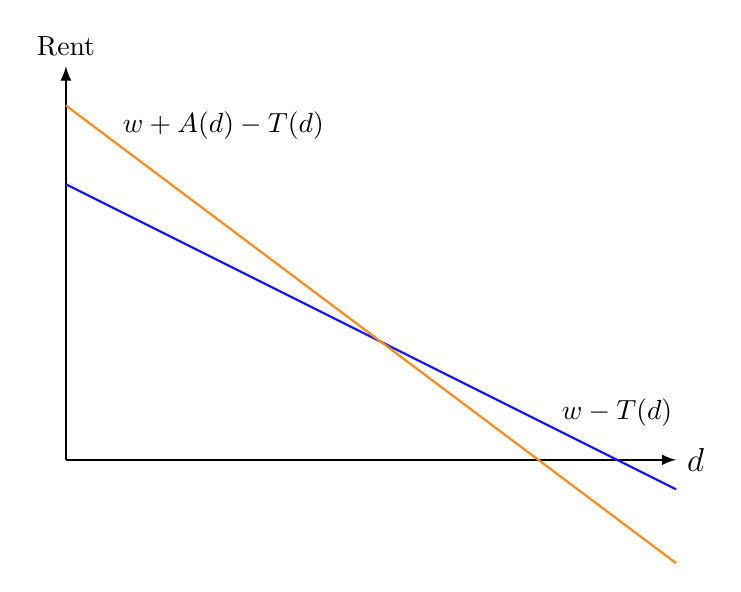
\begin{tikzpicture}[scale=.5]
\def\bndmax{5}        %https://tex.stackexchange.com/questions/68462/filling-a-complex-region-with-tikz
\def\bndmin{0.2}
\def \n {10}
\def \m {15.5}
\def \t {.5}
\def \th {1}
\def \w {7}
\tikzset{func/.style={thick,color=blue!90}}	
\draw [thick, latex-] (0,\n)node[above] {Rent}--(0,0);
\draw [thick, -latex] (0,0)--(\m,0)node[right=.25]{\large $d$};
%\foreach \xi in {0,..., \m} \draw (\xi,0)--(\xi,-.1)node[below=1]{\small$\xi$};
%\foreach \yi in {1,...,\n} \draw (0,\yi)--(-.1,\yi)node[left]{$\yi$};
%%\foreach \i in {1,4,9,16} {
	\draw[func,domain=0:\m] plot [samples=200] (\x,{\w-\t*\x});
%	\draw[func,domain=0:\m, dashed] plot [samples=200] (\x,{\w+\azero-\th*\x+\aprime*\x});

\node at (14,1.2){$w-T(d)$};
\def \azero{2}
\def \aprime {-.25}	
\tikzset{func/.style={thick,color=orange!90}}	
	\draw[func,domain=0:\m] plot [samples=200] (\x,{\w+\azero-\t*\x+\aprime*\x});
\node at (4,8.5){$w +A(d)-T(d)$};
%\node at(-.8,2) [left]{base $2^1=$};
%\node at(-.8,1) [left]{$2^0=$};
%\draw[dotted] (0,2)--(1,2)--(1,0); 
 \end{tikzpicture}
\end{center}
\caption{Rent profile with amenities}
\label{fig-amenity}
\end{figure}

 This model can produce variations on the standard result in the Alonso model. Figure~\ref{fig-amenity} illustrates a linear amenity function, $\mathbb{A}(d|N)= a-b*d$, that is convenient for illustrative purposes.  It shows how a particular amenity function might affect the rent profile, and hence city size and it allows simple experiments with the effect of increasing population on city size, wages and rents. 

In this case, amenity falls below zero in the outer regions of the city and, the geographical size of the city will be smaller. With a linear function, this happens if $\frac{a}{b} < \frac{w}{t}$. (a smaller city would have a secondary effect on wages, since with fewer workers' marginal productivity would be higher and therefore wages would rise. This would partially offset the initial decline in population.)

 There would be a band of land around the city with negative amenity for commuters.\footnote{The very simple graphical result rests on several assumptions - no other housing expense, housing all the same size, wages all equal, preferences identical, transportation costs.}

The far more likely case is that $A(d) > 0$ when $w-T(d)$ falls to zero. In this case there is a band of residents around the city, outside of the population commuting to work. They do not travel to work,  do not collect a wage, but still enjoy the amenity of being close to a city. This might be a population of retired persons enjoying occasional visits and healthcare facilities.


\subsubsection{Neighbourhood amenity}
In Figure~{fig-amenity} the source of the amenity is at the centre of the city. We can easily imagine an amenity profile that is high for some neigbourhoods and lower for others, as in  In Figure~\ref{fig-amenity2}. The jagged area below the orange line is rent accruing to landowners. The variable rent comes not from a desire to be close to the source of the wage income but from household demand for local amenity.  

\begin{figure}[tb]
\begin{center}
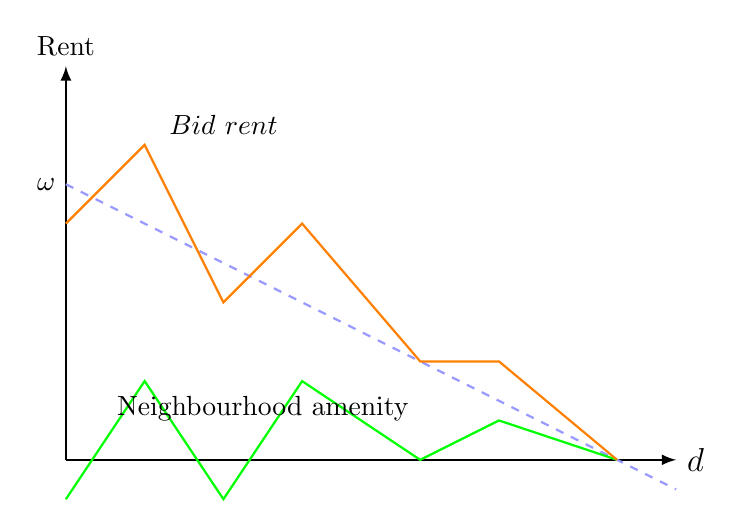
\begin{tikzpicture}[scale=.5]
\def\bndmax{5}        %https://tex.stackexchange.com/questions/68462/filling-a-complex-region-with-tikz
\def\bndmin{0.2}
\def \n {10}
\def \m {15.5}
\def \t {.5}
\def \th {1}
\def \w {7}
\tikzset{func/.style={thick,dashed, color=blue!40}}	
\draw [thick, latex-] (0,\n)node[above] {Rent}--(0,0);
\draw [thick, -latex] (0,0)--(\m,0)node[right=.25]{\large $d$};
% Basic Bid rent,
\node at(-.5,\w) {$\omega$};
\draw[func,domain=0:\m] plot [samples=200] (\x,{\w-\t*\x});
%NEIGBOURHOOD AMENITY
\draw [thick, green] (0,-1)--(2,2)--(4,-1)--(6,2)--(9,0)--(11,1)--(14,0);
\draw [thick, orange] (0,6)--(2,{7-2*.5+2})--(4,7-4*.5 -1)--(6,7-6*.5+2)--(9,7-9*.5)--(11,7-11*.5+1)--(14,7-14*.5);
\node [] at (5,1.3){Neighbourhood amenity};
\def \azero{2}
\def \aprime {-.25}	
% \tikzset{func/.style={thick,color=orange!90}}	
% 	\draw[func,domain=0:\m] plot [samples=200] (\x,{\w+\azero-\t*\x+\aprime*\x});
\node at (4,8.5){$Bid\ rent$};
%\node at(-.8,2) [left]{base $2^1=$};
%\node at(-.8,1) [left]{$2^0=$};
%\draw[dotted] (0,2)--(1,2)--(1,0); 
 \end{tikzpicture}
\end{center}
\caption{Rent profile with neighbourhood amenities}
\label{fig-amenity2}
\end{figure}
Financialization might or might not affect neighbourhood amenity. If it does it might have its effect by changing the ownership mix.

\subsubsection{Public provision of amenities}

Previous sections suggest amenities may work as a wage subsidy, potentially increasing output. Since employers will not willingly pay for urban amenities, some amenities may be financed publicly. It is common to introduce the cost of generating amenities as a tax on residents.  Since public amenities may be \glspl{public good} in the economic sense, the municipal government may be able to achieve significant wage economies with a small public expenditure.

A simple way to incorporate publicly provided amenities to make an amenity function that proportional to a fraction of public revenue, which is a fraction $\tau$ of the land value when municipalities depend on property taxes. Assuming a uniform property tax rate, total property tax revenue in a circular city are approximately $\tau(\phi+2/3 \omega)\pi \frac{\omega}{c}^2$. We can therefore include in the buyer's maximum bid function a fraction if this value. Property investors would not include this amenity component, but it would affect their decisions because amenity raises their net rent.

Notice that because amenity raises property values, in Ontario it does not raise tax revenue because the property tax rate is adjusted to balance the budget. This creates perverse incentives for municipalities \cite{blaisPerverseCitiesHidden2011}.


\subsubsection{An amenity sector}
Producing amenities takes resources. Some fraction of the workforce must be engaged in producing the amenity services. A simple approach would be to assume that the base employment that we consider demands a layer of amenities that represent the additional fraction of the population needed to provide the amenities - say 10\%  

Larger cities can support larger and more varied amenities, so that effect of amenities on property values might be larger in larger cities. At the same time, there are apparently economies of scale in the production of amenities \cite{kaufmannScalingUrbanAmenities2022}. We have no strong prior about how in amenity sector would be affected by finacialization of housing.  An effect might work through changing ownership.


\subsection{Research on amenities}
There is a great deal of research on amenities. In this subsection mention a few that seemed noteworthy. 

Most of the literature on amenities deals with livability and the benefits for the individual. There is a strand in the literature, however, that links amenities to growth. In 1954, for example, Edward Ullman \cite{ullmanAmenitiesFactorRegional1954} published  ``Amenities as a Factor in Regional Growth,'' an article that came to be seen in the geographical literature over the following 50 years as prescient \cite{walcottCommentsEdwardUllman2010} for introducing the notion that amenities could be an important mobility magnet. 

Many have since extended this approach. Richard Florida, in a series of articles and books beginning in 2002 (see \cite{floridaCreativeClassEconomic2014, floridaEconomicGeographyTalent2002, floridaCompetingAgeTalent2005}) examined the notion that urban growth depended on attracting the creative class and that in turn rested in part on the amenities a city offered. A 2008  Statistics Canada study, `Cities and Growth: The Left Brain of North American Cities,' Beckstead et al \ found substantial differences in average growth for cities with higher cultural employment and urban amenities.  Clark et al \cite{clarkAmenitiesDriveUrban2002} argue that much of Chicago's recent growth to 2003  should be attributed to reforms instituted by Mayor Richard M.  Daley explicitly linked to amenities and quality of life issues, including parks and schools. Abouy \cite{albouyWhatAreCities2016} finds that wage and housing cost differences across metropolitan areas are accounted for more by productivity than quality-of-life differences, however. 

 Beckstead et al  \cite{becksteadCitiesGrowthLeft2008} identify amenities with the unexplained variastion in median urban house price after controlling for median household income.\footnote{  The basic premise would be that after conditioning on household income, variation in home prices across cities would be a function of the relative attractiveness of these places. The residuals yield a continuous ranking of cities based on the estimated variation in urban amenities.} Rappaport \cite{rappaportConsumptionAmenitiesCity2008} presents empirical evidence that amenities do support high-density levels, and that amenities cause approximately one-fifth of the cross-sectional variation in metro population density. 


% Molotch's (1976) metaphor suggests that the city is a machine geared to creating growth, with growth loosely defined as the intensification of land use and thus higher rent collections associated professional fees and locally based profits. Many urban economists, planners, and political scientists have made similar arguments (e.g., Bradbury, Downs, & Small, 1982; Mollenkopf, 1983; Stone, 1989). However, a quarter century later in the contemporary competition among US cities, the growth machine model has lost much of its power.
  



%%%%%%%%%%%%%%%%%%%%%%%%%%%%%%%%%%%%%h

\section{Transportation Costs and the Evolution of the City} \label{section-transportation}
Urban transportation is primarily a municipal responsibility.
Transportation improvements that reduce commuting time increase the effective wage. ($\partial{\omega-cd}{c}>0$) but not labour costs, making labour more available for the same wage premium. The effect on rents land rents may vary. If transportation cost keeps falling and lots of land is available, then you don't get strong increases in land prices. If there are strong differentials, that gives you the class result in the city, but doesn't tell you how it would affect it. 


Where you have higher densities, the cities have been collecting more tax per person. 
they overcharge tenants in apartment buildings to subsidize private homes on the edges. 

That would encourage density, which sould encourage density, so you'd have to go to finance.


{\color{red}
One of the first applications of the model was to the effect of a transportation revolution. The advent of first rail transportation and then the automobile radically changed the size, productivity, and population distribution of cities.
periphery available, allowing larger lot sizes and larger homes for those who can afford them.

\begin{figure}[!hb]
\centering
% CHANGING TRANSPORTATION COSTS
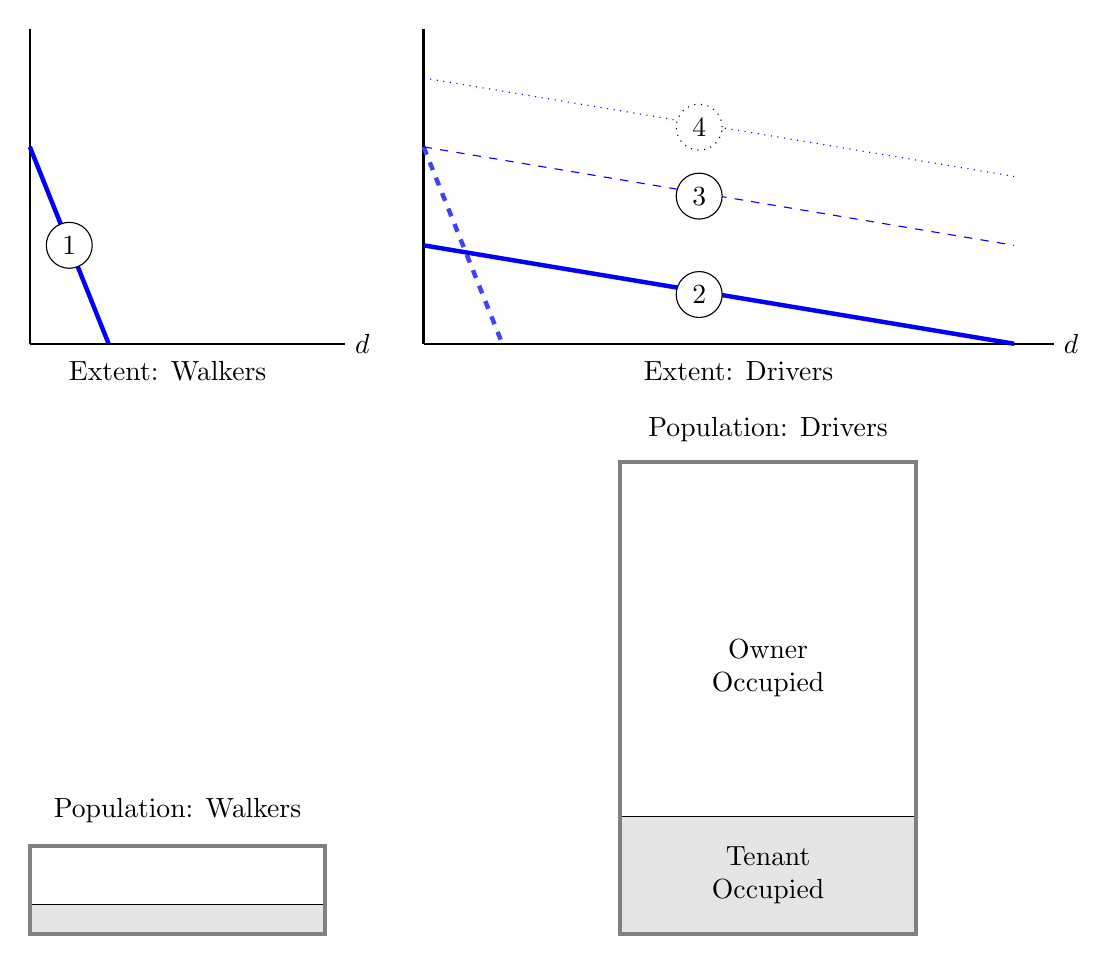
\begin{tikzpicture}[scale=.5]
% EXTENT  BEFORE
\draw[thick](0,0)--(0,8); %Y
\draw[thick](0,0)--(8,0)node[right]{$d$};
\node at (3.5,-.7){Extent: Walkers};
\draw[ultra thick, blue](0,5)--(2,0); 
\node[circle,draw=black, fill=white, inner sep=3pt,minimum size=10pt] (b) at (1,2.5) {1};

% POPULATION BEFORE
\begin{scope}[shift={(0, -15cm)},scale=1.5]%population
\draw [fill=gray!20,] (0,0) rectangle (5,.5); 
\draw[line width= .5mm, black!50] (0,0) rectangle (5,1.5);
\node at (2.5,2.1){Population: Walkers};
\end{scope}

% EXTENT AFTER
\begin{scope}[shift={(10cm, 0)}]
\draw[thick](0,0)--(0,8); %Y
\draw[thick](0,0)--(16,0)node[right]{$d$}; %X
\node at (8,-.7){Extent: Drivers};
\draw[ultra thick, blue!75, dashed](0,5)--(2,0);
\draw[ultra thick, blue](0,2.5)--(15,0);

\node[circle,draw=black, fill=white, inner sep=3pt,minimum size=10pt] (b) at (7,1.25) {2};

\draw[ blue, dashed](0,5)--(15,2.5);
\node[circle,draw=black, fill=white, inner sep=3pt,minimum size=10pt] (b) at (7,3.75) {3};

\draw[ blue, dotted](0,6.75)--(15,4.25);
\node[circle,draw=black, dotted,fill=white, inner sep=3pt,minimum size=10pt] (b) at (7,5.5) {4};
\end{scope}

% POPULATION AFTER
\begin{scope}[shift={(15, -15cm)},scale=1.5]%population
\draw [fill=gray!20,] (0,0) rectangle (5,2); 
\draw[line width= .5mm, black!50] (0,0) rectangle (5,8);
\node at (2.5,8.55){Population: Drivers};
\node at (2.5,4.5)
    [text width=2.4cm, align=center]
    {\baselineskip=20pt Owner Occupied};
%\node at (2,3.3)    [text width=2.4cm]    {\baselineskip=20pt Mortgaged};
\node at (2.5,1)
    [text width=2.4cm, align=center]
    {\baselineskip=20pt Tenant Occupied};
\end{scope}
\label{fig-rent-driving}
\end{tikzpicture}
\caption{Housing tenure post transportation revolution.}
\label{fig-transport-tenure}
\end{figure} 
 
%\input{fig_TransportCost.tex}

The transportation cost revolution brought about by the first street cars and later automobiles made much larger cities possible.  The average walking pace is 2.5 to 4 mph, and new transportation technologies raise this rate by a factor of between five and ten, increasing potential urban area by between twenty-five and one hundred times. 




% THIS IS INTERSTING K.  morgages: Effect of a finbancial instument on urban form!!  suburban flight, second half of the century

%Electric trolleys drew upon manufacturing technology that appeared only in the eighteen eighties and at first only in America. 

%As with other transportation revolutions, institutional as well as technological revolutions were necessary for the interurban phenomenon to succeed.  One such institutional revolution was the creation of the home mortgage in the eighteen eighties.  Another was the development of the public utility, a regulated monopoly, in the earlier twentieth. century.\footnote{https://faculty.washington.edu/jbs/itrans/charge20.htm} The automotive revolution was as important in its way as the coming of the railroads.

%The automobile in time established even more powerful synergies, but they weren't present at the beginning.  Roads suitable for automobiles scarcely existed though new methods of paving utilizing macadam or concrete had recently been invented.  Furthermore, there was no good model in place for road construction.   Unlike the case with either light or heavy rail systems, the vehicles and the road itself were not part of the same corporate entity.       

%Once automotive ownership assumed certain proportions toward the close of the teens of the century, the automobile began to transform the landscape of America in an even more fundamental way than the streetcars had. 

%From the second decade of the twentieth century, the automobile in America has been linked with suburban flight, and when the growth of suburbs reached a crescendo early in the second half of the century, automobile ownership became the norm. 

% Because exurbs are already numerous and growing more so, they place considerable pressure on the Body Politic to ensure that fuel prices remain low, for if prices rise beyond a certain point the exurbanites will be forced to sell out, probably at ruinously low returns because few will choose to live in isolated areas without affordable transportation.  True, exurbs could conceivably be served by public transportation, but only at enormous cost per rider because the population densities are so low in the areas where they are located \dots

% That places the vast suburb dwelling public at risk and the exurbanites most of all.

Initially, rents fell at the centre and rose outside of the original city limits. Lower rents and cheaper suburban housing attract more workers, so that central rents and the land values they support  rise to the original levels and then, because the rising population makes the
city more productive, beyond the original level. 

It  also affected social structure and left indelible marks on the form of cities developing at the time and after. In North America, with large amounts of land, it generated massive urban sprawl, but also made land available for a growing `middle class' of homeowners. This homeowning middle class became the dominant social formation in North 
American society. 

Ultimately the urban expansion generated congestion and rising transportation cost that began to limit urban growth, put upward pressure on  housing costs including transportation, and therefore downward pressure on middle-class effective incomes. Rising congestion costs steepen the rent profile and  reduce the net productivity of cities. Although the process is not a focus of this thesis it represents a relatively simple extension for later work.

\subsection{Differential transportation costs}
 Urbanists agree that before the railroad and the automobile, the extent of a city was roughly determined by how far a person could walk in about an hour. The time and effort cost of transportation determined the size of cities. 
 
 It also affected the distribution of the classes within the city. When everyone walked, the  wealthy may have valued their time more than the poor. In terms of the model, the willingness to pay of the rich would higher  near the core than  the willingness (or ability) to pay of  the poor, but would descend more rapidly with distance
\begin{figure}
\begin{center}
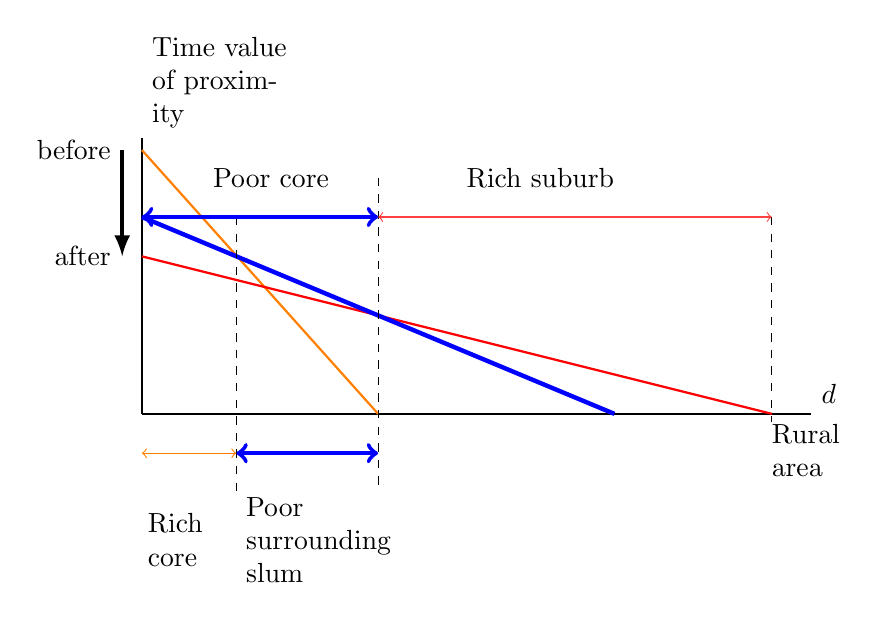
\begin{tikzpicture}[scale=1]
% AXES
\draw[thick](0,0)--(0,3.5)node[above right, text width=1.8cm]{Time  value of proximity}; %Y++
\draw[thick](0,0)--(8.5,0)node[above right]{$d$}node[below, text width =1cm]{Rural area}; 
% BIDS-RENT CURVES
\draw[thick, orange](0,3.35)--(3,0);
\draw[thick, red](0,2)--(8,0);
\draw[ultra thick, blue](0,2.5)--(6,0);

\draw[-latex, ultra thick](-.25,3.35)node[left]{before}--(-.25,2)node[left]{after};
% ZONE DIVISIONS VERTICAL LINES
\draw[dashed](1.2,2.5)--(1.2,-1) ;
\draw[dashed](3,3)--(3,-1) ;
\node at (4,3)[right]{Rich suburb};
\node at (2.5,3)[left]{Poor core};
\draw[dashed](8,2.5)--(8,-.1) ;
%  ARROWS BEFORE
\draw[<->, orange](0,-.5)--(1.2,-.5);
\draw[<->, blue, ultra thick](3,-.5)--(1.2,-.5);
\node[text width =1cm,  left] at (1.2,-1.6){Rich core };
\node[text width =1cm, right] at (1.2,-1.6){Poor \\ surrounding slum};
%  ARROWS AFTER
\draw[<->, blue, ultra thick](0,2.5)--(3,2.5);
\draw[<->, red!75](3,2.5)--(8,2.5);

% \draw[ blue, dashed](0,5)--(15,2.5);
% \node[circle,draw=black, fill=white, inner sep=3pt,minimum size=10pt] (b) at (7,3.75) {3};

% \draw[ blue, dotted](0,6.75)--(15,4.25);
% \node[circle,draw=black, dotted,fill=white, inner sep=3pt,minimum size=10pt] (b) at (7,5.5) {4};
\end{tikzpicture}\end{center}
\caption{A prediction of the basic model: if transportation cost for the rich falls, shifting the orange  bid-rent curve for the rich to the location of the red line, we will see a shift of housing for the rich  from the core to the suburb.}
% \label{fig_fix_my_label}
\end{figure}

 If the technology suddenly provides the rich with commuter trains or automobiles and more attractive sites at the edge of the city, the orange line could drop enough  and become much flatter leading in a flight of the rich to the suburbs, as appears to have happened in many American cities. Lower transportation costs make cheaper land on the edge of the city attractive. This would  offer  more space and the opportunity to build larger homes, a pattern that has emerged in some cities.

\textbf{Experiments}: We first turn off financial  demand and partition the population by wealth and transportation cost to  verify that the predictions made by researchers hold in our model. We then turn financial demand back on  and see if the rate or degree of financialization differs from the base model


\subsection{Municipal costs and revenue}

\begin{figure}
\begin{center}
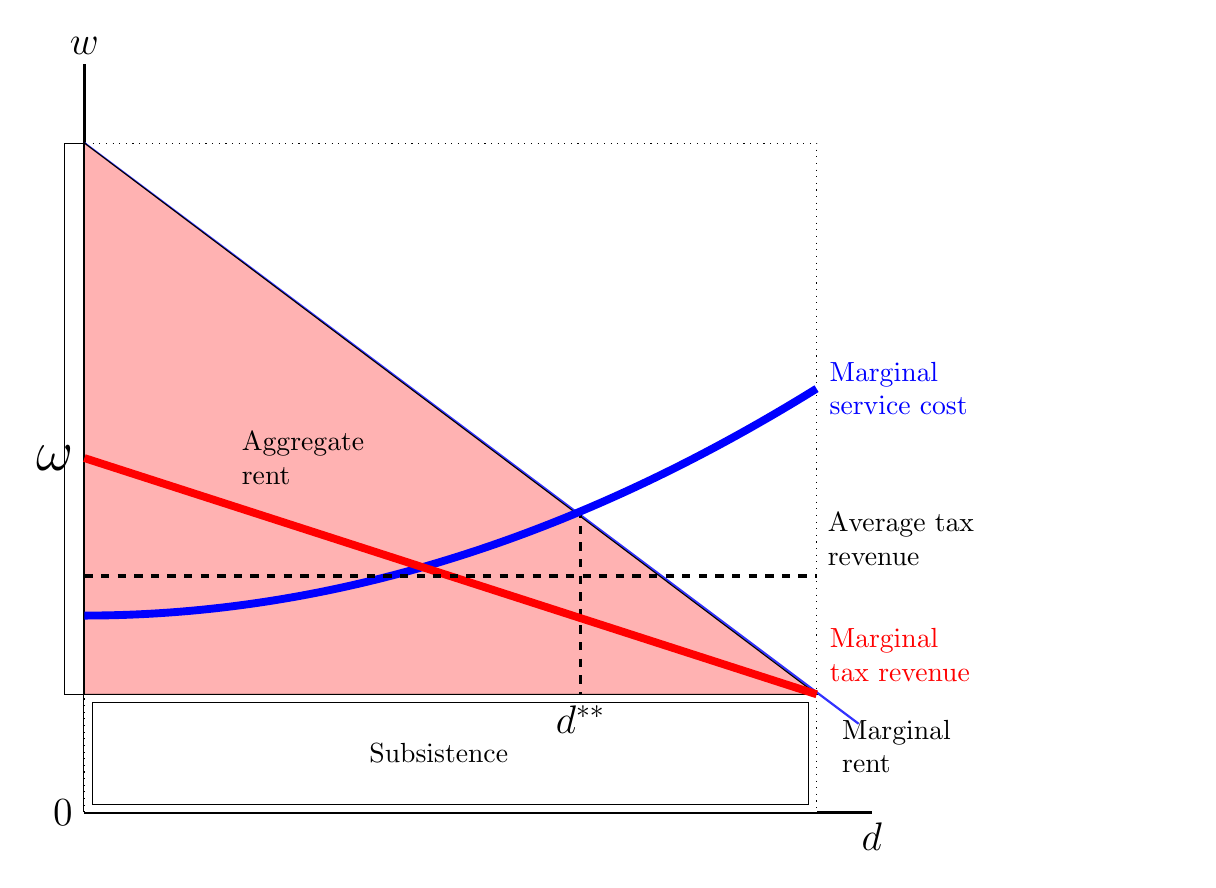
\begin{tikzpicture}[scale=1]
\def\bndmax{5}        %https://tex.stackexchange.com/questions/68462/filling-a-complex-region-with-tikz
\def\bndmin{0.2}
\def \n {8}  % height of y axis
\def \d {10}  % length  of x axis
\def \t {.75}  %  cost of transportation per unit x
\def \th {1}   %
\def \w {7}    %  wage premium
\def \om{1.5}%  omega =rural wage Zero for urban population
\def \azero{2}
\def \aprime {-.0}	
\tikzset{func/.style={thick,color=blue!80}}	
\draw [thick] (0,-\om) --(\d,-\om)node[below]{\Large $d$};  			% Zero for rural population
\draw [thick] (0,-\om)node[left=.5]{\Large $0$} --(0,\n)node[above]{\Large $w$};	% Y axis

%\draw [thick] (0,0)node[left=.5]{ subsistance}--(\d,0);
\node[left=.25] at (0,3){\huge $\omega$};
%\node[left=.25] at (0,\w+.3){subsistence plus};
%\node[left=.25] at (0,\w-.4){wage premium};	

\draw[fill=white, white] (0.1,-0.1) rectangle (14,-\om+.1);
\draw [] (-.25, 0) rectangle(.25, \w);%fill=green!30!blue!30
\node[right] at  (.25, \w/2){Added Productivity};
%\draw [ thick, ->](11.3,-\om/2)--(13, -\om/2)node [right] {\Large $d$};
\draw[fill=blue!40] (0.1,-0.1) rectangle (9.2,-\om+.1);

\draw[fill=black!0, dotted] (0,-\om) rectangle (9.30,\w);% new product repeat
\draw[func, domain=0:\w/\t+.5] plot [samples=200] (\x,{\w-\t*\x}); %rent profile
\draw[fill=blue!0] (0.1,-0.1) rectangle (9.2,-\om+.1);
\node at (4.5,-\om/2){Subsistence};
\draw[fill=red!30,] (0.,0.)--(0,7)--(9.30,0.)--cycle;% Rent \w-.2
\node[text width=2cm] at (3.,3){Aggregate \\rent}; 		%Rent 
%\node at (5.8,5.7)[]{\Large Transportation};
\node at (6.3,4.8)[white]{\Large expenditure};
\draw[ line width=.5mm, dashed] (6.3,2.35)--(6.3,0)node[below ]{\Large $d^{**}$};

\draw[func, domain=0:9.3, line width=1mm,blue, text width=2cm] plot [samples=200] (\x,{1+\x^2/30})node[right]{Marginal\\ service cost};
\draw[ line width=1mm, red] (0,3)--(9.3,0)node[above right, text width=3cm ]{Marginal\\tax revenue};
\node at (9.5, -.2)[below right, text width=2cm]{Marginal rent};

\draw[ line width=.5mm, dashed] (0,1.5)--(9.3,1.5)node[above right, text width=2.5cm ]{Average tax revenue};
%GRID
%\draw[step=1cm,gray,very thin] (0,0) grid (10,10);
\end{tikzpicture}
\end{center}
\caption[The Alonso model with municipal costs and revenue.]{The Alonso model \gls{rent profile}, as illustrated in Figure~\ref{fig-alonso-simple}, with cost and municipal costs and revenue added.} %service fees added.}
\label{fig-municipal-costs}
\end{figure}
 

 Two stylized facts should be noticed. The first is that the marginal cost of servicing generally rises with the distance from the centre. Figure illustrates the general form of servicing costs, but not the relative scales of rent and servicing costs. When this observation is combined with the \gls{Henry George Theorem} the conclusion is that the optimal size of the city  is at  $d^{**}$, where marginal service cost intersects with the marginal increase in total urban rent.  Walter Christaller, 1933

The second stylized fact is that property taxes, which are generally  fixed as a share of property value, decline as the distance from the centre increases. Figure~\ref{fig-municipal-costs} illustrates the general form of tax liabilities, although it does not  accurately represent their relationship to rent or  servicing costs. This implies that in many or most urban situations the residents at the outer edges pay less than the average amount in property tax per unit of land, but cost  the community budget more than the average amount. In essence, the central city subsidizes the suburbs. (see Perverse Cities \ref{blaisPerverseCitiesHidden2011}). This arrangement is both economically inefficient and unfair, but it has been built into the fiscal structure of cities largely as a result of automobile-based urban growth. It is likely that this fiscal misallocation saps some of the potential productivity growth of cities. Property taxation reduces the market value of properties, but it also funds services and amenities that increase the value of properties. 

Both servicing and taxation effects are more variable and than the simple model suggests.  One conclusion urban theorists draw based on variants of the Alonso model is that because property owners in the low-density urban margin are subsidized,  the subsidy is likely to create serious fiscal problems for municipalities in the long-term and result in serious inefficiency in land use.

Political opposition is essentially rent seeking.

}